% See exam.cls and examdoc.tex for the license information
\documentclass[12pt, answers]{exam}

\usepackage{amssymb}
\usepackage{makeidx}
\usepackage{amsmath}
\usepackage{graphicx}
\usepackage{caption}
\usepackage{tabulary}
\usepackage{color}
\usepackage{multicol}
%\usepackage{multirow}
%\usepackage{enumerate}

\usepackage{array}
\newcolumntype{C}[1]{>{\centering\let\newline\\\arraybackslash\hspace{0pt}}m{#1}}

\addpoints

% In case we're not using hyperref.sty:
\providecommand{\texorpdfstring}[2]{#1}
% The following can be used in \section commands
% without generating pdf warnings:
\newcommand{\bs}{\texorpdfstring{\char`\\}{}}

\makeindex

\newcommand{\indc}[1]{\index{#1@\texttt{\char`\\#1}}}
\newcommand{\indcsub}[2]{\index{#1@\texttt{\char`\\#1}!#2}}
\newcommand{\indcstart}[1]{\index{#1@\texttt{\char`\\#1}|(}}
\newcommand{\indcstop}[1]{\index{#1@\texttt{\char`\\#1}|)}}

\newcommand{\indt}[1]{\index{#1@\texttt{#1}}}
\newcommand{\indtsub}[2]{\index{#1@\texttt{#1}!#2}}
\newcommand{\indtstart}[1]{\index{#1@\texttt{#1}|(}}
\newcommand{\indtstop}[1]{\index{#1@\texttt{#1}|)}}

\extraheadheight{-.4in}

\pagestyle{headandfoot}
%\extraheadheight{.2 in}
\firstpageheader{}{}{}
\runningheader{}{}{}
\firstpagefooter{}{Global pairwise alignment}{Page \thepage\ of \numpages}
\firstpagefootrule
\runningfooter{}{Global pairwise alignment}{Page \thepage\ of \numpages}
\runningfootrule

%---------------------------------------------------------------------

\shadedsolutions
%\noprintanswers
\definecolor{SolutionColor}{rgb}{0.8,0.9,1}

\setcounter{section}{1}

\begin{document}

\section{Exercise solutions -- Global pairwise alignment}

%---------------------------------------------------------------------
\begin{questions}

%%% Question 1
\question \textbf{Pairwise alignments}
  
Pairwise alignments are two aligned sequences of DNA, RNA, or protein. DNA and RNA sequences consist of four different nucleotides, whereas protein sequences consist of 20 different amino acids. The  ``-'' sign is used to represent a blank or a gap, which indicates an insertion or a deletion from one sequence to the other.

Use the simple scoring scheme and calcuate the score of the following alignments.

\textbf{Scoring scheme: }\\
\null \quad $R_{ab}$ = 1 for a = b \\ 
\null \quad $R_{ab}$ = 0 for a $\neq$ b \\ 
\null \quad g = 1  

\vspace{0.1 in}

\begin{parts}

%% (a)
  \part
  Alignment 1
  \begin{verbatim}
    q: ATGCT
    d: CA--T \end{verbatim}
    
  \begin{solution}[0.35 in]
  -1
  \end{solution}

%% (b)
  \part
  Alignment 2
  \begin{verbatim}
    q: CAGCT
    d: C-A-T \end{verbatim}
  
  \begin{solution}[0.35 in]
  0
  \end{solution}
    
  \vspace{0.1 in}

\end{parts}

%%% Question 2
\question \textbf{Brute force approach}
  
A brute force approach can be used to find the optimal alignment. Use the sequences $q$ and $d$ below and answer the questions.

\begin{multicols}{2}
Sequences:
\begin{verbatim}
  q: CG, d: AC
\end{verbatim}
\vfill\null
\columnbreak

\noindent Scoring scheme: \\ 
\null \quad $R_{ab}$ = 1 for a = b \\ 
\null \quad $R_{ab}$ = 0 for a $\neq$ b \\ 
\null \quad g = 1

\end{multicols} 

\vspace{0.1 in}

\begin{parts}

%% (a)
  \part
  Identify all possible alignments.
  
  \begin{solution}[2.5 in]
  \begin{verbatim}
  l = 4  CG--    C-G-    C--G    -CG-    -C-G    --CG
         --AC    -A-C    -AC-    A--C    A-C-    AC--

  l = 3  CG-   CG-   C-G    C-G    -CG    -CG
         A-C   -AC   AC-    -AC    A-C    AC-

  l = 2  CG
         AC	
  \end{verbatim}
  \end{solution}

%% (b)
  \part
  Identify the optimal alignment with its score.
  
  \begin{solution}[0.75 in]
  \begin{verbatim}
  CG
  AC    Score: 0
  \end{verbatim}

  \end{solution}
    
  \vspace{0.1 in}

\end{parts}


%%% Question 3
\question \textbf{Table representation}
  
An alignment can be represented as a table with arrows. Vertical and horizontal arrows indicate gaps, while diagonal arrows indicate matches and mismatches.

Identify the alignment that corresponds to the arrows in the following tables.
\medskip 

\begin{parts}

%% (a)
\part Table 1

\begin{figure}[h]
  \centering
      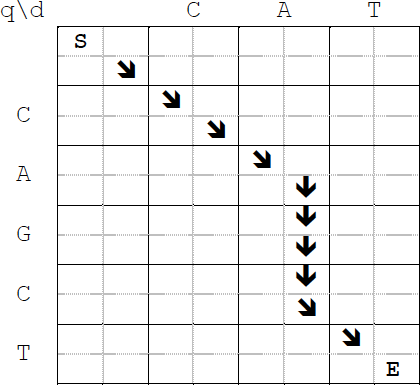
\includegraphics[width=0.325 \textwidth]{fig02/alignment_table_exercise_1.png}
\end{figure}

\begin{solution}[0.75 in]
\begin{verbatim}
  q: CAGCT
  d: CA--T
\end{verbatim}
\end{solution}

%% (b)
\part Table 2 

\begin{figure}[!h]
  \centering
      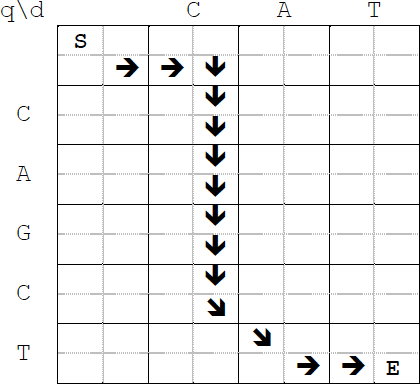
\includegraphics[width=0.325 \textwidth]{fig02/alignment_table_exercise_2.png}
\end{figure}

\begin{solution}[0.75 in]
\begin{verbatim}
  q: -CAGCT-
  d: C----AT
\end{verbatim}
\end{solution}

\end{parts}

\pagebreak



\end{questions}
%---------------------------------------------------------------------
       
\end{document}

